\documentclass[10pt,tikz,border=3pt]{standalone}
\usepackage{amsmath,amssymb}
\usetikzlibrary{arrows.meta}
\definecolor{boundary}{RGB}{55,126,184}
\definecolor{direct}{RGB}{44,154,57}
\definecolor{onebounce}{RGB}{213,52,45}
\definecolor{twobounce}{RGB}{117,76,166}
\definecolor{sourcec}{RGB}{230,126,20}
\definecolor{graystem}{RGB}{145,145,145}
\begin{document}
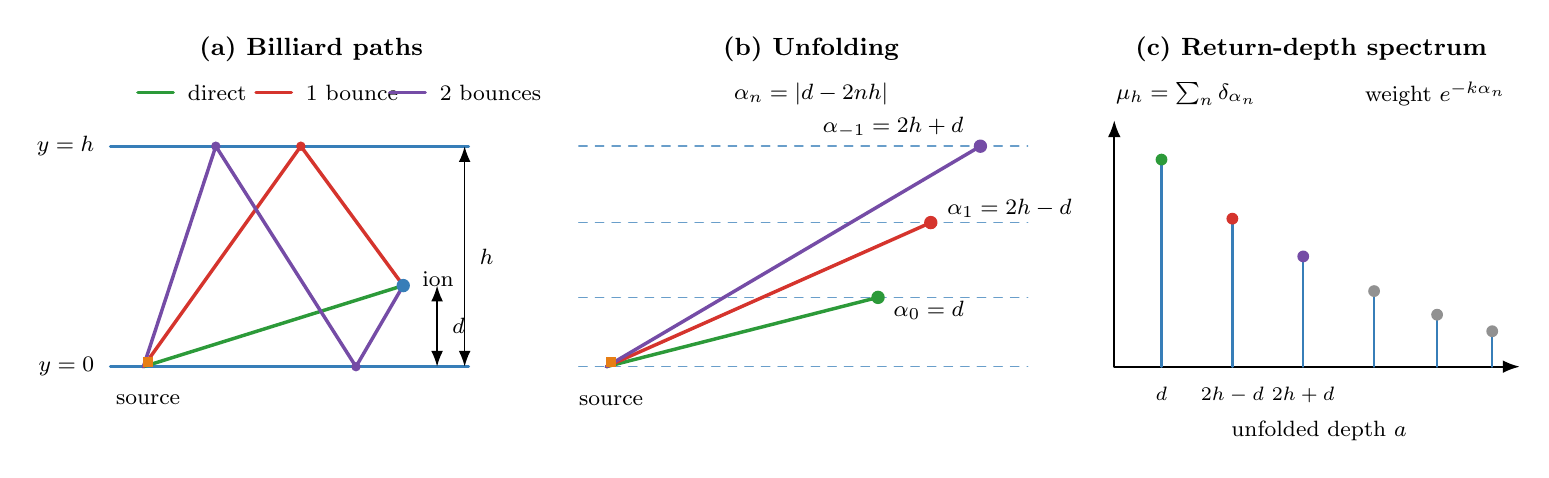
\begin{tikzpicture}[x=1cm,y=1cm,line cap=round,line join=round,>=Latex]
\tikzset{lab/.style={font=\footnotesize}, smalllab/.style={font=\scriptsize}, paneltitle/.style={font=\small\bfseries}}

\node[paneltitle] at (2.85,4.85) {(a) Billiard paths};
\draw[direct,line width=1.2pt] (0.65,4.30)--(1.10,4.30);
\node[lab,anchor=west] at (1.16,4.30) {direct};
\draw[onebounce,line width=1.2pt] (2.15,4.30)--(2.60,4.30);
\node[lab,anchor=west] at (2.66,4.30) {1 bounce};
\draw[twobounce,line width=1.2pt] (3.85,4.30)--(4.30,4.30);
\node[lab,anchor=west] at (4.36,4.30) {2 bounces};
\draw[boundary,line width=1.1pt] (0.30,0.82)--(4.85,0.82);
\draw[boundary,line width=1.1pt] (0.30,3.62)--(4.85,3.62);
\node[lab,anchor=east] at (0.22,3.62) {$y=h$};
\node[lab,anchor=east] at (0.22,0.82) {$y=0$};
\coordinate (S) at (0.72,0.82);
\coordinate (I) at (4.02,1.85);
\coordinate (R1) at (2.72,3.62);
\coordinate (R2a) at (1.64,3.62);
\coordinate (R2b) at (3.42,0.82);
\draw[direct,line width=1.25pt] (S)--(I);
\draw[onebounce,line width=1.25pt] (S)--(R1)--(I);
\draw[twobounce,line width=1.25pt] (S)--(R2a)--(R2b)--(I);
\fill[sourcec] (S) rectangle ++(0.12,0.12);
\fill[boundary] (I) circle (0.085);
\fill[onebounce] (R1) circle (0.06);
\fill[twobounce] (R2a) circle (0.06);
\fill[twobounce] (R2b) circle (0.06);
\node[lab,anchor=north] at (0.78,0.58) {source};
\node[lab,anchor=west] at (4.14,1.93) {ion};
\draw[<->,line width=0.6pt] (4.45,0.82)--(4.45,1.85);
\node[lab,anchor=west] at (4.52,1.34) {$d$};
\draw[<->,line width=0.6pt] (4.80,0.82)--(4.80,3.62);
\node[lab,anchor=west] at (4.87,2.22) {$h$};

\node[paneltitle] at (9.20,4.85) {(b) Unfolding};
\node[lab] at (9.20,4.28) {$\alpha_n=|d-2nh|$};
\foreach \yy in {0.82,1.70,2.65,3.62} {
  \draw[boundary,dashed,line width=0.55pt,opacity=0.75] (6.25,\yy)--(11.95,\yy);
}
\coordinate (S2) at (6.60,0.82);
\coordinate (A0) at (10.05,1.70);
\coordinate (A1) at (10.72,2.65);
\coordinate (Am1) at (11.35,3.62);
\draw[direct,line width=1.25pt] (S2)--(A0);
\draw[onebounce,line width=1.25pt] (S2)--(A1);
\draw[twobounce,line width=1.25pt] (S2)--(Am1);
\fill[sourcec] (S2) rectangle ++(0.12,0.12);
\fill[direct] (A0) circle (0.085);
\fill[onebounce] (A1) circle (0.085);
\fill[twobounce] (Am1) circle (0.085);
\node[lab,anchor=north] at (6.66,0.57) {source};
\node[lab,anchor=west,fill=white,inner sep=1.2pt] at (10.20,1.53) {$\alpha_0=d$};
\node[lab,anchor=west,fill=white,inner sep=1.2pt] at (10.88,2.83) {$\alpha_1=2h-d$};
\node[lab,anchor=east,fill=white,inner sep=1.2pt] at (11.18,3.86) {$\alpha_{-1}=2h+d$};

\node[paneltitle] at (15.55,4.85) {(c) Return-depth spectrum};
\node[lab,anchor=west] at (12.95,4.28) {$\mu_h=\sum_n\delta_{\alpha_n}$};
\node[lab,anchor=east] at (18.15,4.28) {weight $e^{-k\alpha_n}$};
\draw[line width=0.7pt,->] (13.05,0.82)--(18.20,0.82);
\draw[line width=0.7pt,->] (13.05,0.82)--(13.05,3.95);
\foreach \xx/\yy/\cc in {13.65/3.45/direct,14.55/2.70/onebounce,15.45/2.22/twobounce,16.35/1.78/graystem,17.15/1.48/graystem,17.85/1.27/graystem} {
  \draw[boundary,line width=0.9pt] (\xx,0.82)--(\xx,\yy);
  \fill[\cc] (\xx,\yy) circle (0.075);
}
\node[smalllab,anchor=north] at (13.65,0.68) {$d$};
\node[smalllab,anchor=north] at (14.55,0.68) {$2h-d$};
\node[smalllab,anchor=north] at (15.45,0.68) {$2h+d$};
\node[lab,anchor=north] at (15.65,0.25) {unfolded depth $a$};
\end{tikzpicture}
\end{document}
